\documentclass[10pt]{beamer}
\usetheme[background=light,block=fill,progressbar=foot]{metropolis}
%\usepackage[UTF8]{ctex}
\usepackage{graphicx}
\usepackage{caption}
\usepackage{bm}
\newcommand{\supercite}[1]{\textsuperscript{\textsuperscript{\cite{#1}}}}
%\usefonttheme[onlymath]{serif}

\begin{document}
	\title{Deep Learning Book}
	\subtitle{Chapter 6 \\ Deep Feedforward Networks}
	\author{Botian Shi \\ botianshi@bit.edu.cn}
	
	\date{\today}
	\begin{frame}[plain]
		\titlepage
	\end{frame}
	
	\begin{frame}{Feedforward Networks}
		
		\begin{itemize}
			\item A type of neural network
				\begin{itemize}
					\item \emph{Deep feedforward network}
					\item \emph{feedforward neural network}
					\item \emph{multilayer perceptron (MLP)}
				\end{itemize}
			\item For a classifier, $y = f^{\,*}(\bm{x})$ maps an input $\bm{x}$ to category $\bm{y}$
			\item Defines a mapping:
					\begin{center}
						$\bm{y}=f(\bm{x};\bm{\theta})$
					\end{center}
			\item Learns the best approximation of $f^{\,*}$ with parameter $\bm{\theta}$
			\item Feedforward only, no feedback connections.
			\item The basis of many applications.
		\end{itemize}
	\end{frame}

	\begin{frame}{Feedforward networks are ...}
		\begin{enumerate}
			\item Extreme important.
			\item Stepping stone on the path to recurrent neural networks.
		\end{enumerate}
		\begin{exampleblock}{Example: convolutional neural network}
			\begin{figure}
				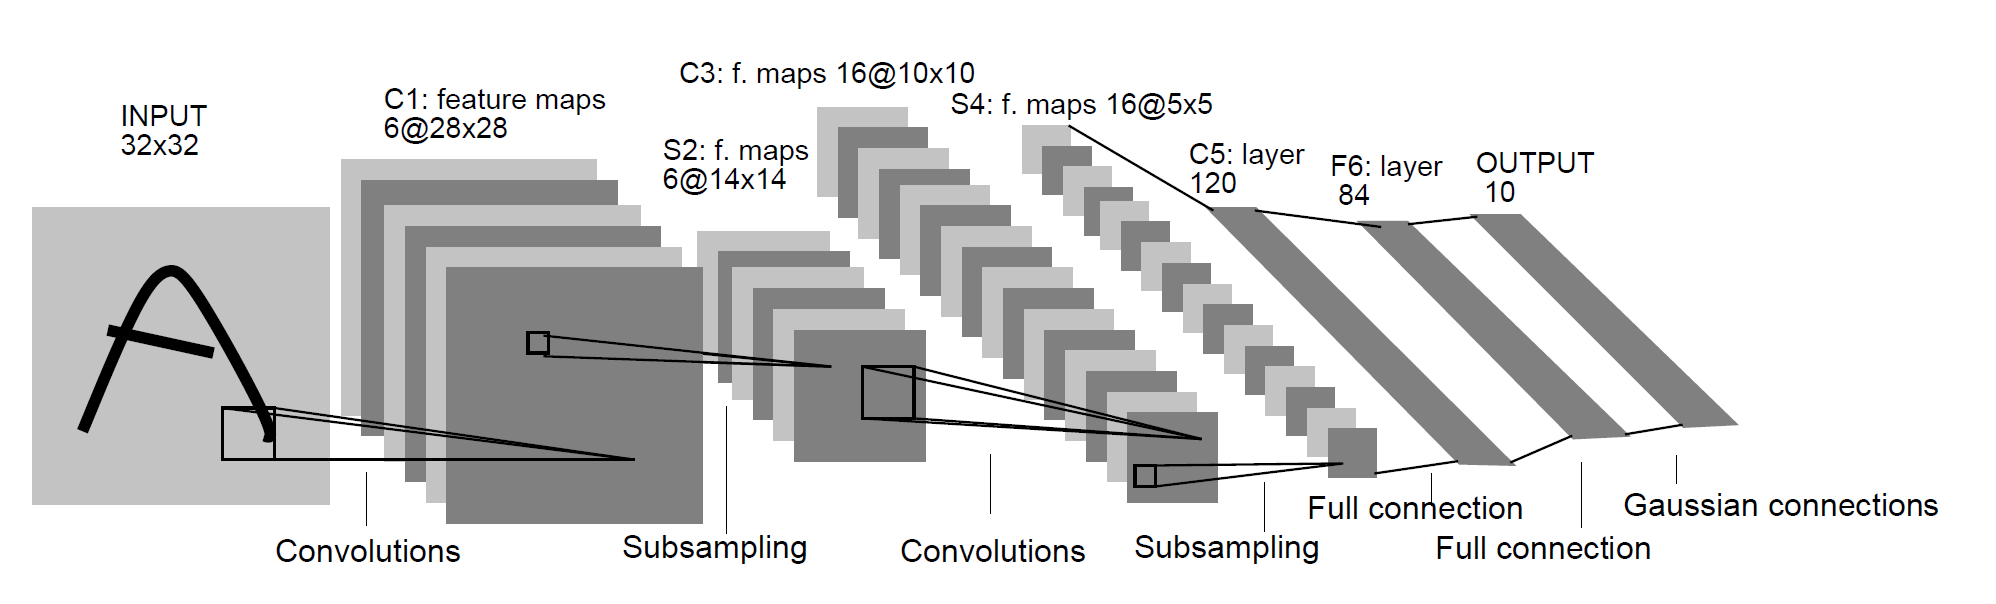
\includegraphics[width=25em]{figures/lenet-5.png}
				\caption{A type of convolutional neural network: LeNet-5\supercite{lecun1998gradient}}
			\end{figure}
		\end{exampleblock}
	\end{frame}

	\begin{frame}{Multilayer Perceptron}
		\begin{columns}[T,onlytextwidth]
			\column{0.7\textwidth}
			\begin{itemize}
				\item Why called \emph{networks}?
				\begin{itemize}
					\item Composing together many different functions.
					\item Model is associated with a DAG describing the composition.
					\begin{equation*}
					f(\bm{x}) = f^{\,(3)\,}(f^{\,(2)\,}(f^{\,(1)\,}(\bm{x})))
					\end{equation*}
					\item $f^{\,(1)\,}$ called first layer of the network
					\item $f^{\,(2)\,}$ called second layer, and so on
					\item $f^{\,(2)\,}$ called output layer
				\end{itemize}
			\end{itemize}
			\column{0.3\textwidth}
			\begin{figure}
				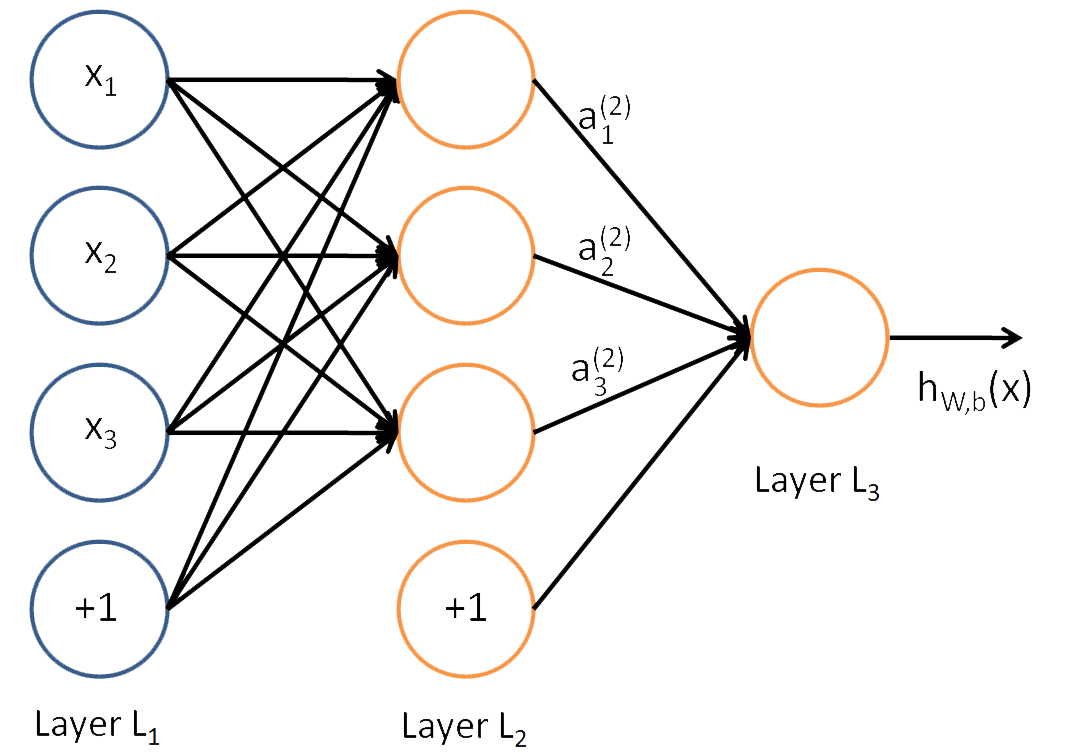
\includegraphics[width=10em]{figures/multilayer-perceptron.png}
				\caption{\\ An example of MLP  (from \href{http://ufldl.stanford.edu/wiki/index.php/File:Network331.png}{UFLDL})}
			\end{figure}
		\end{columns}
		\begin{itemize}
			\item During training, we drive $f\,(\bm{x})$ to match $f^{\,*}(\bm{x})$
			\item Each example $\bm{x}$ is accompanied by a label $y\approx f^{\,*}(\bm{x})$
			\item At each point $\bm{x}$, network must produce a value that is close to $\bm{y}$.
			\item The learning algorithm must decide how to use those layers to produce the desired output.
			\item Layers between input and output layer are called \emph{hidden layer}.
		\end{itemize}
	\end{frame}

	\begin{frame}{The \emph{NEURAL} network}
		\begin{itemize}
			\item Inspired by neuroscience.
			\begin{columns}
				\column{0.5\textwidth}
				\begin{figure}
					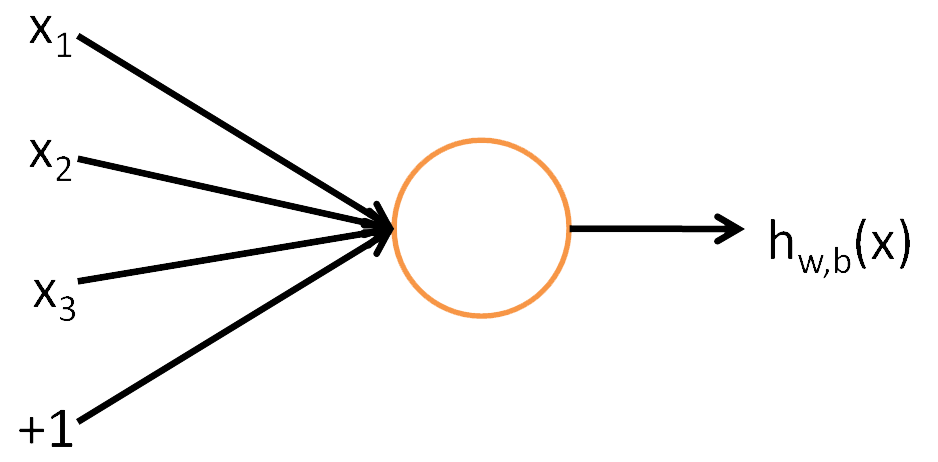
\includegraphics[height=5em]{figures/neuron.png}
					\caption{Neuron (from \href{http://deeplearning.stanford.edu/wiki/index.php/File:SingleNeuron.png}{UFLDL})}
				\end{figure}
			
				\column{0.5\textwidth}
				\begin{figure}
					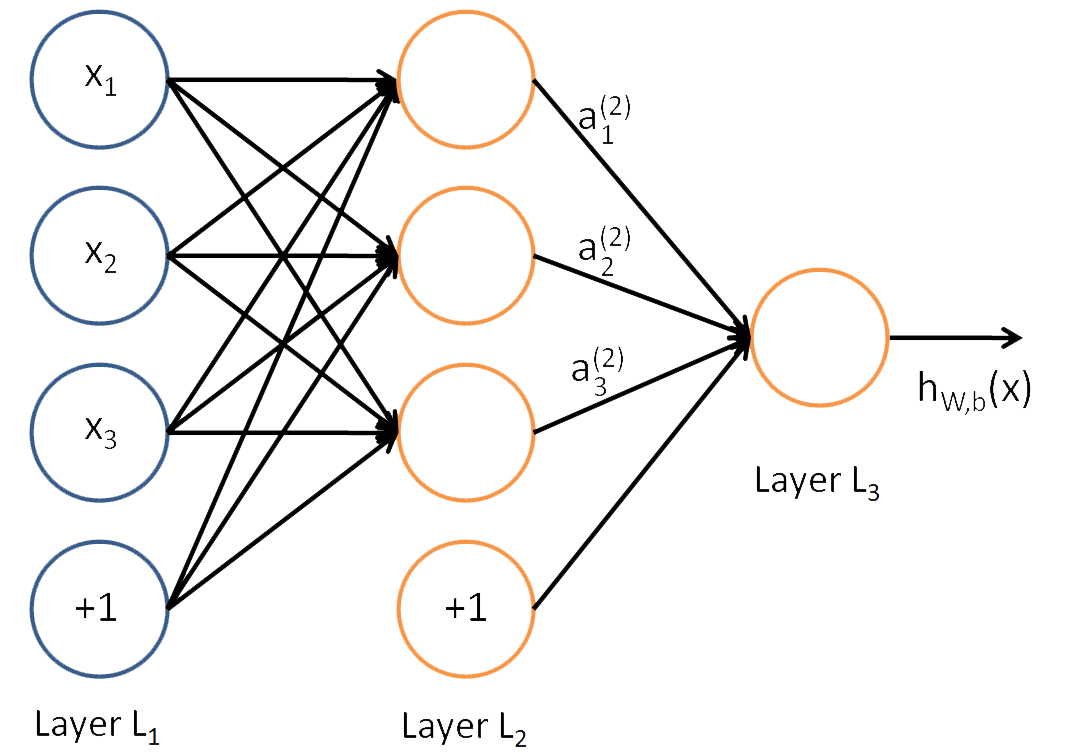
\includegraphics[height=5em]{figures/multilayer-perceptron.png}
					\caption{MLP (from \href{http://ufldl.stanford.edu/wiki/index.php/File:Network331.png}{UFLDL})}
				\end{figure}
					
			\end{columns}
			\item Each hidden layer is vector-valued. The dimensionality of these hidden layers determines the \emph{width} of the model.
			\item Each element of the vector may be interpreted as a neuron.
			\item Layer consist of many \emph{units} that act in parallel, each representing a vector-to-scalar function.
			\item Each unit resembles a neuron that receives input from many other units and computes its own activation value.
		\end{itemize}
	\end{frame}

	\begin{frame}{The \emph{NEURAL} network}
		\begin{itemize}
			\item The idea of using many layers of vector-valued representation is drawn from neuroscience.
			\item Modern neural network research $\ne$ perfectly model the brain.
			\item Feedforward networks $\approx$ function approximation machines.
			\item Inspired by brain, rather than model a brain.
		\end{itemize}
	\end{frame}

	\begin{frame}{}
		内容...
	\end{frame}

	\begin{frame}[allowframebreaks]{References}
		\bibliography{Chap6}
		\bibliographystyle{abbrv}
	\end{frame}

\end{document}